\documentclass{beamer}
\usepackage{amsmath}
%\usepackage{beamerthemesplit} % new 
\usetheme{Madrid}
\usefonttheme[onlymath]{serif}
\setbeamertemplate{frametitle}[default][center] %center slide titles

%My commands
\newcommand{\ket}[1]{\left| #1 \right>}
\newcommand{\bra}[1]{\left< #1 \right|}
\newcommand{\braket}[2]{\left<\left. #1 \right| #2 \right>}
\newcommand{\ak}{a_k}
\newcommand{\akd}{a_k^\dagger}
\newcommand{\akb}{a_{\bar{k}}}
\newcommand{\akbd}{a_{\bar{k}}^\dagger}
\newcommand{\ai}{a_i}
\newcommand{\aid}{a_i^\dagger}
\newcommand{\aib}{a_{\bar{i}}}
\newcommand{\aibd}{a_{\bar{i}}^\dagger}
\newcommand{\alk}{\alpha_k}
\newcommand{\alkd}{\alpha_k^\dagger}
\newcommand{\alkb}{\alpha_{\bar{k}}}
\newcommand{\alkbd}{\alpha_{\bar{k}}^\dagger}
\newcommand{\ali}{\alpha_i}
\newcommand{\alid}{\alpha_i^\dagger}
\newcommand{\alib}{\alpha_{\bar{i}}}
\newcommand{\alibd}{\alpha_{\bar{i}}^\dagger}
\newcommand{\uk}{\mathrm{u}_k}
\newcommand{\vk}{\mathrm{v}_k}
\newcommand{\hBE}{\hat{\mathcal{E}}}
\newcommand{\tBE}{\widetilde{\mathcal{E}}}

\begin{document}
\title{Notes on Siemens Ch. 8.4}
\author{Cody Petrie} 
\date{\today} 

%start slides
\frame{\titlepage}

\frame{\frametitle{Harmonic Vibrations in the Random Phase Approximation}
\begin{itemize}
   \item We are going to look at small vibrations around equilibrium ($Q^0$).
   \item Follow the cranking model which says that $Q_\alpha = Q_\alpha(t)$, and then solve for the equations of motion for $Q_\alpha(t)$.
   \item He says that this chapter treats $Q_\alpha$ as the main dynamic variable. Elevating it above $\mathbf{r}_i$ and $\mathbf{p}_i$ comes at the expense of a classical treatment of $Q_\alpha$.
\end{itemize}
}

\frame{\frametitle{Harmonic Vibrations in the Random Phase Approximation}
\framesubtitle{Constructing the Single-particle Hamiltonian}
\begin{itemize}
   \item The HF mean field expectation value double counts the two-body potential terms so we can't use those.
   \begin{equation}
      \sum\limits_{j=1}^A \varepsilon_j = \bra{\psi_{HF}}\sum\limits_{i=1}^A \frac{p_i^2}{2m_N} \ket{\psi_{HF}} + \bra{\psi_{HF}}\sum\limits_{ij}V(\mathbf{r}_i-\mathbf{r}_j)\ket{\psi_{HF}}
   \end{equation}
   where
   \begin{equation}\begin{split}
      \bra{\psi_{HF}}H\ket{\psi_{HF}} = \bra{\psi_{HF}} & \sum\limits_{i=1}^A \frac{p_i^2}{2m_N} \ket{\psi_{HF}} \\ &+ \frac{1}{2}\bra{\psi_{HF}}\sum\limits_{ij}V(\mathbf{r}_i-\mathbf{r}_j)\ket{\psi_{HF}}
   \end{split}\end{equation}
   
\end{itemize}
}

\frame{\frametitle{Harmonic Vibrations in the Random Phase Approximation}
\framesubtitle{Constructing the Single-particle Hamiltonian}
\begin{itemize}
   \item The (incorrect) independent-particle model (ipm) energy is given by $\hBE = \sum\limits_{i=1}^A \hat{\varepsilon}_i$.
   \item Strutinsky, in chapter 5, found a correction to the ipm energy in terms of the liquid-drop energy and the smoothed single-particle energy $\tBE$.
   \begin{equation}
      \bra{\psi_{HF}}H\ket{\psi_{HF}} = \hBE + \delta \tBE
   \end{equation}
   \begin{equation}
      \delta \tBE(Q_\alpha) = \tilde{E}-\tBE = -B_{LD}-\tBE
   \end{equation}
   \item Which gives us the single-particle hamiltonian
   \begin{equation}
      H_{sp} = \sum\limits_{i=1}^A H^{sp}(\mathbf{r}_i,\mathbf{p}_I,\{Q_\alpha\}) = \delta\tBE(\{Q_\alpha\}) + \sum\limits_{i=1}^A H^{ipm}(\mathbf{r}_i,\mathbf{p}_I,\{Q_\alpha\})
   \end{equation}
   \item Notice that the additional term doesn't depend on the intrinsic coordinates, $\mathbf{r}$ and $\mathbf{p}$.
\end{itemize}
}

\frame{\frametitle{Harmonic Vibrations in the Random Phase Approximation}
\framesubtitle{Constructing the Single-particle Hamiltonian}
\begin{itemize}
   \item Equations 8.2.3 and 8.2.15 are then just changed by a constant value
   \begin{align}
      H_0^{sp} &= H^{ipm}(\mathbf{r},\mathbf{p},\{Q_\alpha^0\}) + \delta \tBE(\{Q_\alpha^0\})/A \\
      F_\mu^{sp} &= \frac{\partial H^{sp}}{\partial Q_\mu} \Bigr \rvert_{\{Q\alpha=Q\alpha^0\}} = F_\mu^{ipm} + \frac{\partial}{\partial A_\mu^0} \frac{\delta \tBE(\{Q_\alpha^0\})}{A}
   \end{align}
   Where the $F$ is the form factor
   \item This will shift $F_\mu$ and the single-particle energies by a uniform amount, but will not effect the response function because it does not depend on the diagonal elements.
\end{itemize}
}

\frame{\frametitle{Harmonic Vibrations in the Random Phase Approximation}
\framesubtitle{Constructing the Equation of Motion}
\begin{itemize}
   \item We now use this single-particle hamiltonian, the fact that $\left<H_{sp}\right>$ is conserved, and Ehrenfest's theorem to get the equations of motion.
   \item Ehrenfest's theorem: $\frac{d}{dt}\left<A\right> = \frac{1}{i\hbar}\left<\left[A,H\right]\right> + \left<\frac{\partial A}{\partial t}\right>$
   \begin{align}
      0&=\frac{d}{dt}\bra{\psi(t)}H_{sp}\ket{\psi(t)} = \bra{\psi(t)\frac{}{}}\frac{\partial}{\partial t} H_{sp}(\{Q_\alpha(t)\})\ket{\psi(t)\frac{}{}} \\
      &=\sum_\mu \frac{dQ_\mu}{dt}\bra{\psi(t)\frac{}{}}\frac{\partial H_{sp}}{\partial t}\ket{\psi(t)\frac{}{}}
   \label{equ:8.4.9}
   \end{align}
   \item The solution to this for any dynamic $Q_\alpha$ implies that
   \begin{equation}
      \bra{\psi(t)\frac{}{}}\frac{\partial H_{sp}}{\partial Q_\mu}\ket{\psi(t)\frac{}{}} = 0
      \label{equ:condition}
   \end{equation}
\end{itemize}
}

\frame{\frametitle{Harmonic Vibrations in the Random Phase Approximation}
\framesubtitle{Constructing the Equation of Motion}
\begin{itemize}
   \item Now remember that we are doing this for small oscillations around $Q_\mu^0$. So let's expand to second order in $Q_\mu-Q_\mu^0$.
   \begin{equation}\begin{split}
      H_{sp} \approx \sum\limits_i H_0^{sp}(\mathbf{r}_i,\mathbf{p}_i) + \sum_\mu(Q_\mu-Q_\mu^0)\sum_iF_\mu^{sp}(\mathbf{r}_i,\mathbf{p}_i,\{Q_\alpha^0\}) \\
      + \frac{1}{2}\sum\limits_{\mu,\nu}(Q_\mu-Q_\mu^0)(Q_\nu-Q_\nu^0)\sum\limits_i\frac{\partial^2 H^{sp}}{\partial Q_\mu \partial Q_\nu}(\mathbf{r}_i,\mathbf{p}_i,\{Q_\alpha^0\})
   \end{split}\end{equation}
   \item Now let's force equation~\ref{equ:condition} to be zero.
   \begin{equation}\begin{split}
      -\bra{\psi(t)\frac{}{}}\frac{\partial H_{sp}}{\partial Q_\mu} \ket{\psi(t)\frac{}{}} = 0 \approx -\bra{\psi(t)\frac{}{}}\sum\limits_i F_\mu^{sp}(\mathbf{r}_i,\mathbf{p}_i,\{Q_\alpha^0\}\ket{\psi(t)\frac{}{}} \\
      - \sum\limits_\nu (Q_\nu(t)-Q_\nu(t)^0)\bra{\psi(t)\frac{}{}}\sum\limits_i\frac{\partial^2 H^{sp}}{\partial Q_\mu \partial Q_\nu}(\mathbf{r}_i,\mathbf{p}_i,\{Q_\alpha^0\}) \ket{\psi(t)\frac{}{}}
   \end{split}\end{equation}
\end{itemize}
}

\frame{\frametitle{Harmonic Vibrations in the Random Phase Approximation}
\framesubtitle{Constructing the Equation of Motion}
\begin{itemize}
   \item Now using equation 8.4.12 and adding the linear term from above we get can find the equation of motion for $Q_\nu$.
   \begin{equation}\begin{split}
      0=\int\limits_{-\infty}^\infty dt' \sum\limits_\nu \widetilde{\chi}^{ipm}_{\mu\nu}(t-t')(Q_\nu(t')-Q^0_\nu) - \bra{gs\frac{}{}}\sum\limits_i F_\mu^{sp}\ket{gs\frac{}{}} \\
      + \sum\limits_\nu \kappa_{\mu\nu}(Q_\nu(t)-Q_\nu^0)
   \end{split}\end{equation}
   where
   \begin{equation}
      \kappa_{\mu\nu} = \bra{gs\frac{}{}}\sum\limits_i
\frac{\partial^2 H^{sp}}{\partial Q_\mu \partial Q_\nu}(\mathbf{r}_i,\mathbf{p}_i,\{Q_\alpha^0\})\ket{gs\frac{}{}}.
   \end{equation}
\end{itemize}
}

\frame{\frametitle{Harmonic Vibrations in the Random Phase Approximation}
\framesubtitle{Small-amplitude Vibrational Solutions}
\begin{itemize}
   \item How are we going to solve this?
   \item Let's assume small-vibrations around the equilibrium $\{Q_\alpha^0\}$, where
   \begin{equation}
      \bra{gs\frac{}{}}\sum\limits_iF_\mu^{sp}(\{Q_\alpha^0\})\ket{gs\frac{}{}}=0.
   \end{equation}
   \item Now let's try a solution of the form $Q_\nu(t) = Q_\nu^0+A_\nu^n e^{-i\omega_n t + \phi}$.
   \item This is a solution given the condition (eigenvalue equation)
   \begin{equation}
      \sum\limits_\nu \left[\kappa_{\mu\nu}+\chi_{\mu\nu}^{ipm}(\omega_n)\right]A_\nu^n = 0
   \end{equation}
   \item This is a solution given the condition
   \begin{equation}
      \mathrm{det}\left|\kappa_{\mu\nu} + \chi_{\mu\nu}^{ipm}(\omega_n)\right| = 0
      \label{equ:8.4.16}
   \end{equation}
   \item This is called the characteristic equation of the RPA (Random Phase Approximation).
\end{itemize}
}

\frame{\frametitle{Harmonic Vibrations in the Random Phase Approximation}
\framesubtitle{Small-amplitude Vibrational Solutions}
\begin{itemize}
   \item Let's try to understand the RPA eigenvalue equation by assuming that both $\kappa_{\mu\nu}$ and $\chi_{\mu\nu}^{ipm}$ are diagonal.
   \item If we do this we get solutions when $\chi_\mu^{ipm}=-\kappa_\mu$, where these are the $\mu^{\mathrm{th}}$ diagonal elements.
   \item From the previous equations of the ipm (8.2.10,8.2.11,8.1.18) we get
   \begin{equation}\begin{split}
      \chi_\mu^{ipm}(\omega) = &\sum\limits_{jk} \frac{N_{jk}}{\hbar}\left|\bra{j}F_\mu^{ipm}\ket{k}\right|^2 \\
      &\left[\frac{2\omega_{kj}P}{\omega_{kj}^2 - \omega^2} + i\pi\left[\delta(\omega-\omega_{kj}) - \delta(\omega-\omega_{kj})\right]\right].
   \end{split}\end{equation}
   \item Since $\chi_\mu^{ipm'}$ is the real part, when $\kappa_\mu$ is real we get
   \begin{equation}
      \chi_\mu^{ipm'}(\omega_n) = \sum\limits_{jk}\frac{N_{jk}}{\hbar}\left|\bra{j}F_\mu^{ipm}\ket{k}\right|^2\left[\frac{2\omega_{kj}}{\omega_{kj}^2-\omega_n^2}\right] = -\kappa_\mu
   \end{equation}
\end{itemize}
}

\frame{\frametitle{Harmonic Vibrations in the Random Phase Approximation}
\framesubtitle{Small-amplitude Vibrational Solutions}
\begin{figure}
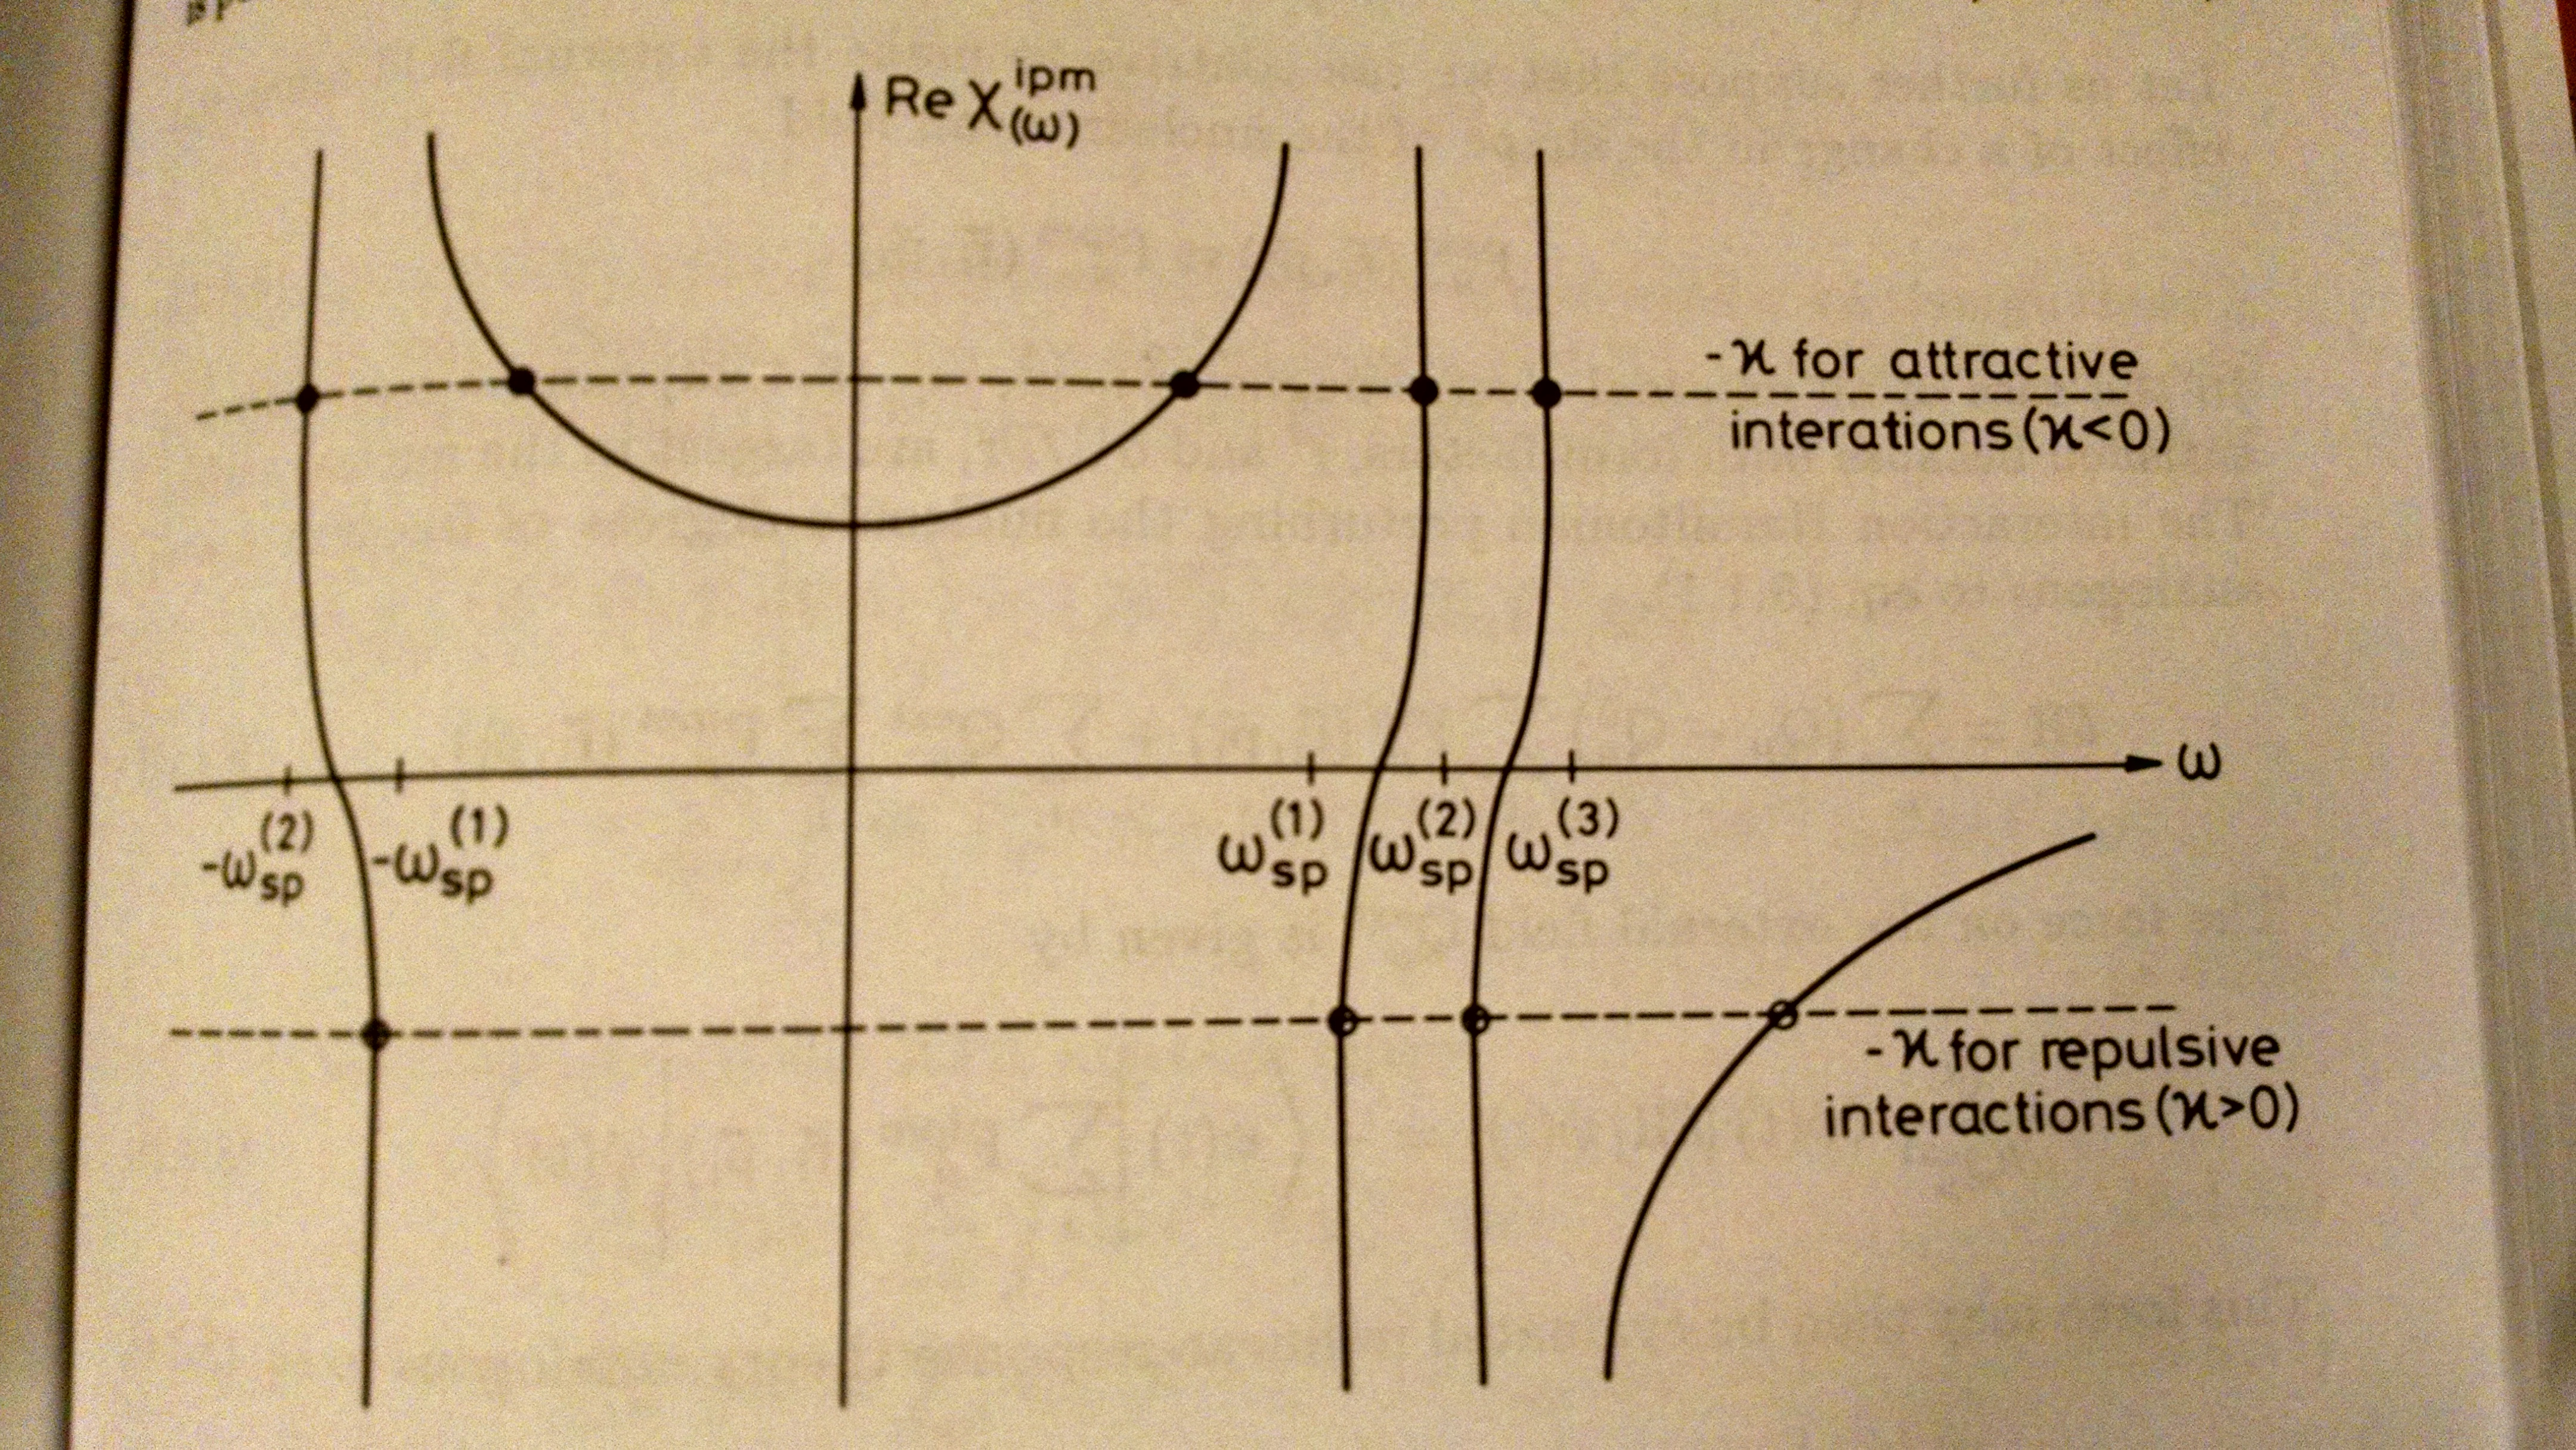
\includegraphics[width=\textwidth]{fig8_4.jpg}
\end{figure}
}

\frame{\frametitle{Harmonic Vibrations in the Random Phase Approximation}
\framesubtitle{RPA Response to an External Field}
\begin{itemize}
   \item Let's add in an weak external field with parameters $Q_\mu^{ext}(t)$ and see how the nucleus responds.
   \begin{align}
      H=\sum\limits_i H^{sp}(\mathbf{r}_i,&\mathbf{p}_i,\{Q_\alpha(t)\}) + H^{ext}(\mathbf{r}_i,\mathbf{p}_i,\{Q_\mu^{ext}(t)\}) \\
      H^{ext} &= \sum\limits_\mu F_\mu^{ext}(\mathbf{r}_i,\mathbf{p}_i)Q_\mu^{ext}(t)
   \end{align}
   \item Not to simplify things let's assume we can make the external field look like the mean field.
   \begin{equation}
      F_\mu^{ext}(\mathbf{r}_i,\mathbf{p}_i) \approx F_\mu^{ipm}(\mathbf{r}_i,\mathbf{p}_i)
   \end{equation}
\end{itemize}
}

\frame{\frametitle{Harmonic Vibrations in the Random Phase Approximation}
\framesubtitle{RPA Response to an External Field}
\begin{itemize}
   \item Now we can write the perturbing hamiltonian as
   \begin{equation}
      \delta H = \sum\limits_\mu (Q_\mu-Q_\mu^0) \sum\limits_i F_\mu^{sp}(\mathbf{r}_i,\mathbf{p}_i) + \sum\limits_\mu Q_\mu^{ext}\sum\limits_iF_\mu^{ipm}(\mathbf{r}_i,\mathbf{p}_i)
   \end{equation}
   \item Then the force on the external field is
   \begin{equation}
      -\frac{\partial}{\partial Q_\mu^{ext}}\bra{\psi(t)}\delta H\ket{\psi(t)} = -\bra{\psi(t)\frac{}{}}\sum\limits_iF_\mu^{ipm}(\mathbf{r}_i,\mathbf{p}_i)\ket{\psi(t)\frac{}{}}
   \end{equation}
   \item With linear-response theory (see eq. 8.1.6) this becomes
   \begin{equation}\begin{split}
      \bra{\psi(t)\frac{}{}}\sum\limits_iF_\mu^{ipm}(\mathbf{r}_i,\mathbf{p}_i)\ket{\psi(t)\frac{}{}} = \bra{gs\frac{}{}}\sum\limits_i F_\mu^{ipm}(\mathbf{r}_i,\mathbf{p}_i)\ket{gs\frac{}{}}\\
      -\sum\limits_\nu\int\limits_{-\infty}^\infty dt' \tilde{\chi}_{\mu\nu}^{ipm}(t-t')\left[Q_\nu(t')-Q_\nu^0+Q_\nu^{ext}(t')\right]
   \end{split}\end{equation}
\end{itemize}
}

\frame{\frametitle{Harmonic Vibrations in the Random Phase Approximation}
\framesubtitle{RPA Response to an External Field}
\begin{itemize}
   \item We can now use equation 8.1.11 to calculate the rate of change of the energy due to this external field.
   \begin{equation}\begin{split}
      \frac{dE}{dt} &= \sum\limits_\mu\frac{dQ_\mu^{ext}}{dt}\bra{\psi(t)\frac{}{}}\sum\limits_i F_\mu^{ipm}(\mathbf{r}_i,\mathbf{p}_i)\ket{\psi(t)\frac{}{}} \\
      &\equiv \frac{d}{dt}\bra{\psi(t)} H(t) \ket{\psi(t)}
   \end{split}\end{equation}
   \item Using Ehrenfest's theorem again we can write
   \begin{equation}\begin{split}
      \frac{d}{dt}\bra{\psi(t)}& H(t) \ket{\psi(t)} = \bra{\psi(t)\frac{}{}}\frac{\partial H}{\partial t}\ket{\psi(t)\frac{}{}} \\
       &= \sum\limits_\mu \frac{dQ_\mu^{ext}}{dt}\bra{\psi(t)\frac{}{}}\sum\limits_i F_\mu^{ipm}(\mathbf{r}_i,\mathbf{p}_i)\ket{\psi(t)\frac{}{}} \\
      & \qquad+ \sum\limits_\mu \frac{dQ_\mu}{dt}\bra{\psi(t)\frac{}{}}\frac{\partial H_{sp}}{\partial Q_\mu} \ket{\psi(t)\frac{}{}}
   \end{split}\end{equation}
\end{itemize}
}

\frame{\frametitle{Harmonic Vibrations in the Random Phase Approximation}
\framesubtitle{RPA Response to an External Field}
\begin{itemize}
   \item Putting these two equations together we see that equation~\ref{equ:8.4.9} (8.4.9) is still truei even with the external field.
   \item After some computation it can be shown that
   \begin{equation}\begin{split}
      \bra{\psi(t)\frac{}{}}\sum\limits_i F_\mu^{ipm}(\mathbf{r}_i,\mathbf{p}_i)\ket{\psi(t)\frac{}{}} = \bra{gs\frac{}{}}\sum\limits_i F_\mu^{ipm}(\mathbf{r}_i,\mathbf{p}_i)\ket{gs\frac{}{}} \\
      -\sum\limits_\nu \int\limits_{-\infty}^{\infty} dt'\tilde{\chi}_{\mu\nu}^{RPA}(t-t')(Q_\nu^{ext}(t') + \sum\limits_\sigma(\kappa^{-1})_{\nu\sigma}\bra{gs}F_\sigma\ket{gs},
   \end{split}\end{equation}
   which shows the RPA responce tensor to be
   \begin{align}
      \tilde{\chi}_{\mu\nu}^{RPA}(t) &= \frac{1}{2\omega}\int d\omega e^{-i\omega t}\chi_{\mu\nu}^{RPA}(\omega) \\
      \tilde{\chi}_{\mu\nu}^{RPA}(\omega) &= \sum\limits_{\rho\lambda}\kappa_{\mu\lambda}[\kappa+\chi^{ipm}(\omega)]^{-1}_{\lambda\rho} \chi_{\rho\nu}^{ipm}(\omega).
   \end{align}
\end{itemize}
}

\frame{\frametitle{Harmonic Vibrations in the Random Phase Approximation}
\framesubtitle{RPA Response to an External Field}
\begin{itemize}
   \item This RPA response tensor describes the total force on the external field due to the nucleons' rearrangement.
   \item Analagous to dielectric theory in E\&M
   \begin{itemize}
      \item $Q^{ext} \rightarrow D$
      \item $Q-Q^0 \rightarrow P$
      \item $Q+Q^{ext} \rightarrow E$
   \end{itemize}
   \item So the polarization (response) tensor, which is proportional to the matrix in equation~\ref{equ:8.4.16} whose determinant is zero, which implies that $\chi_{\mu\nu}^{RPA}$ has poles at $\omega_n$.
   \begin{align}
      \chi_{\mu\nu}^{RPA}(\omega) = \sum\limits_n\left[\frac{P}{\omega_n-\omega} - i\pi\delta(\omega_n-\omega)\right] \\
      D_{\mu\nu}^n = -\lim_{\epsilon\rightarrow 0} \epsilon \sum\limits_{\rho\lambda}[\kappa+\chi^{ipm}(\omega_n+\epsilon)]^{-1}_{\lambda\rho}\chi_{\rho\nu}^{ipm}(\omega_n)
   \end{align}
\end{itemize}
}

\frame{\frametitle{Harmonic Vibrations in the Random Phase Approximation}
\framesubtitle{RPA Response to an External Field}
\begin{itemize}
   \item Simplifying to one variable to analyze the nature of the singularities, we get
   \begin{equation}
      D^n = \frac{\kappa^2}{\partial \chi^{ipm'}/\partial\omega}\bigg\rvert_{\omega_n},
   \end{equation}
   where $D^n$ tells how easy it is to excite the nucleus with an external field of $\omega_n$.
   \item He says that, from figure 8.4, these are the eigenfrequencies that lie farthest from the ipm excited energies. The states are the states when the external field acts on all particles equally, and are called ``collective" states.
\end{itemize}
}

\frame{\frametitle{Harmonic Vibrations in the Random Phase Approximation}
\framesubtitle{Vibrational Parameters: the Coupling Constant and the Sum Rule}
\begin{itemize}
   \item An important step in calculating the collective vibrational motion of nuclei is to determine the $Q$'s and the associated form factors,
   \begin{equation}
      F_\mu^{sp} = \frac{\partial H^{sp}}{\partial Q_\mu} \bigg\rvert_{Q_\alpha = Q_\alpha^0}
   \end{equation}
   \item To do this we need to know the Hamiltonian and associated states and energies, $H^{sp}_0\ket{k} = \hat{\varepsilon}_k\ket{k}$.
   \item One way to do this is to calculate $\kappa$ using the definition.
   \begin{equation}
      \kappa_{\mu\nu} \equiv -\bra{gs\frac{}{}}\frac{\partial^2 H_{sp}}{\partial Q_\mu \partial Q_\nu}\bigg\rvert_{Q_\alpha=Q_\alpha^0}\ket{gs\frac{}{}}
   \end{equation}
\end{itemize}
}

\frame{\frametitle{Harmonic Vibrations in the Random Phase Approximation}
\framesubtitle{Vibrational Parameters: the Coupling Constant and the Sum Rule}
\begin{itemize}
   \item Now, like Bohr and Mottelson, let's use the ipm potential (8.3.1), and look at vibrations about a spherical equilibrium to obtain an estimate of the coupling constant in 8.4.20.
   \begin{align}
      \kappa_l &= -R(A)^2 \int\limits_0^\infty dr r^2 \hat{n}(r)\left(\frac{\partial^2\hat{U}}{\partial r^2}+\frac{2}{R(A)}\frac{\partial\hat{U}}{\partial r}\right) \\
      &\approx -R(A)^2 \int\limits_0^\infty dr r^2 \hat{n}(r) \left(\frac{\partial^2\hat{U}}{\partial r^2} + \frac{2}{r}\frac{\partial \hat{U}}{\partial r}\right) \\
      &= \frac{R(A)^2}{4\pi} \int d^3 \mathbf{r} \nabla \hat{n}(\mathbf{r}) \cdot \nabla \hat{U}(\mathbf{r})
   \end{align}
   \item It turns out that $\kappa$ is very sensative to the choice of $H^{sp}(Q)$, and requires a second order approximation, whereas $F_\mu^{sp}$ only requires a first order approximation.
\end{itemize}
}

\frame{\frametitle{Harmonic Vibrations in the Random Phase Approximation}
\framesubtitle{Vibrational Parameters: the Coupling Constant and the Sum Rule}
\begin{itemize}
   \item 8.4.20 was a second order approximation. There is another way to calculate $\kappa_{\mu\nu}$ that only requires first order variables.
   \item This method involves determining the shape of the potential from the density, as we did before.
   \item First, given a density distribution due to vibrational motion, we calculate the mean value of $F_\mu^{sp}$ and the parameters $Q_\mu-Q_\mu^0$. We can then use equation 8.4.12 to first order to get
   \begin{equation}
      \kappa_{\mu\nu} = \frac{\partial}{\partial Q_\nu} \bra{\{Q_\alpha\}}\sum\limits_i F_\mu^{sp} \ket{\{Q_\alpha\}}\rvert_{Q_\alpha^0}
   \end{equation}
\end{itemize}
}

\frame{\frametitle{Harmonic Vibrations in the Random Phase Approximation}
\framesubtitle{Vibrational Parameters: the Coupling Constant and the Sum Rule}
\begin{itemize}
   \item Let's apply this to a deformed Woods-Saxon potential. Use equations 5.3.1 to describe the deformation in both $\hat{U}(\mathbf{r})$ and the density $\hat{n}(\mathbf{r})$.
   \item Assuming that $F_{\mu\nu}$ is real tells us that $m=0$. Also note that $F_{l0}^{ipm}$ is proportional to $Y_l^0(\theta,\phi)$ (8.4.38), so the only part of the density that contributes to the expectation value is the part with the same angular dependence,
   \begin{equation}
      \delta n_{l0}(\mathbf{r}) = -\alpha_{l0}Y_l^0(\theta,\phi)R(A)\frac{\partial}{\partial r} \hat{n}(\mathbf{r})
   \end{equation}
   \item Now using equations 8.3.2 and 8.4.39 we get get
   \begin{equation}
      \kappa_l = \frac{\partial}{\partial \alpha_{l0}} \int\limits_0^\infty f^2 dr \frac{\partial \hat{U}}{\partial r}\frac{\partial \hat{n}}{\partial r} \cdot \int d\Omega Y_l^0(\theta,\phi)^2\alpha_{l0}R(A)^2,
   \end{equation}
   which is the same as equation 8.4.37 (which was second order).
\end{itemize}
}

\frame{\frametitle{Harmonic Vibrations in the Random Phase Approximation}
\framesubtitle{Vibrational Parameters: the Coupling Constant and the Sum Rule}
\begin{itemize}
   \item Now we define a quantity called the energy-weighted sum rule,
   \begin{align}
      S_{\mu\nu} &= \frac{1}{2} \bra{gs\frac{}{}} \left[\sum\limits_i F_\mu^{sp}, \left[H_{sp}(\{Q_\alpha^0\}),\sum\limits_iF_\nu^{sp}\right]\right]\ket{gs\frac{}{}} \\
      &= \sum_n(E_n-E_0)\bra{gs\frac{}{}}\sum\limits_i F_\mu^{sp}\ket{n\frac{}{}}\bra{n\frac{}{}}\sum\limits_i F_\nu^{sp}\ket{gs\frac{}{}}.
   \end{align}
   \item Comparing this with equation 8.1.24 we can write this as
   \begin{equation}
      S_{\mu\nu} = \frac{\hbar^2}{2\pi}\int\limits_{-\infty}^\infty d\omega \chi_{\mu\nu}^{ipm''}(\omega)\cdot\omega.
   \end{equation}
\end{itemize}
}

\frame{\frametitle{Harmonic Vibrations in the Random Phase Approximation}
\framesubtitle{Vibrational Parameters: the Coupling Constant and the Sum Rule}
\begin{itemize}
   \item From the hamiltonian from the RPA (8.4.11)
   \begin{equation}\begin{split}
      H_{sp}^{RPA} \approx &\sum\limits_i H_0^{sp}(\mathbf{r}_i,\mathbf{p}_i) + \sum_\mu(Q_\mu-Q_\mu^0)\sum_iF_\mu^{sp}(\mathbf{r}_i,\mathbf{p}_i,\{Q_\alpha^0\}) \\
      &- \frac{1}{2}\sum\limits_{\mu\nu}\kappa_{\mu\nu}(Q_\mu-Q_\mu^0)(Q_\nu-Q_\nu^0)
   \end{split}\end{equation}
   we see that the commutator in $S_{\mu\nu}$ would be the same wether we use $H_{sp}(\{Q_\alpha\})$ or $H_{sp}(\{Q_\alpha^0\})$, and thus we can write
   \begin{align}
      S_{\mu\nu} &= \frac{\hbar^2}{2\pi}\int\limits_{-\infty}^\infty d\omega \chi_{\mu\nu}^{RPA''}(\omega)\cdot\omega \\
      &= \hbar^2 \sum\limits_{\omega_n > 0} D_{\mu\nu}^n\cdot \omega_n
   \end{align}
\end{itemize}
}

\frame{\frametitle{Harmonic Vibrations in the Random Phase Approximation}
\framesubtitle{Vibrational Parameters: the Coupling Constant and the Sum Rule}
\begin{itemize}
   \item $S$ is interesting because it only depends on the nuclear ground state, $F_\mu^{sp}$ and $H_{sp}$, and the right-hand side depends on the individual RPA vibrational solutions. Thus when you only know some of these, you can use it to deduce if the rest are ``collective" (contribute) or not.
   \item From the inverse FT we can write
   \begin{equation}
      S_{\mu\nu} = \hbar^2\frac{d}{dt}\tilde{\chi}_{\mu\nu}^{RPA}(t)\big\rvert_{t=0} = \hbar^2\frac{d}{dt}\tilde{\chi}_{\mu\nu}^{ipm}(t)\big\rvert_{t=0}.
   \end{equation}
   \item From this we can see that $S_{\mu\nu}$ represents the short-time behavior of the response function $\tilde{\chi}_{\mu\nu}$ and that it's the same for ipm and RPA.
   \item Meaning that the interactions of the field only affect the long-time behavior of the response.
\end{itemize}
}

\end{document}
